\documentclass[thesis.tex]{subfiles}

\begin{document}
\chapter{Method}
This chapter discusses the practical implementation of objectives described in introduction. It contains FBA pipeline implementation details, description of the steps taken for performing CoBundleMap extension, as well as caveats and problems encountered during the whole working process.

\section{FBA pipeline}
First step of extending CoBundleMap with new metrics is to implement a mechanism which would perform computation of FDC. For building such pipeline we will refer to original papers about AFD \cite{afd2012Raffelt} and FDC \cite{fdcAndFBA2017Raffelt} as well as official Mrtrix documentation \cite{mrtrixDocu, mrtrixGeneral2019}.

\subsection{Computing fiber orientation distributions}
First step of the FBA pipeline is the calculation of a single unique subjects-averaged response function. Using such a function for computing fiber orientation distributions is the central idea of fixel-based analysis. It allows us to interpret acquired apparent fiber density values as a metric being measured in units of this common function, which is crucial for executing inter-subject comparison.

We will be using existing response functions, which were calculated with \textit{dwi2response} \cite{dwi2response} during the \textit{preprocessing} step of CoBundleMap for each subject and compute their mean by utilizing \textit{average\_response} command from MRtrix package. It is worth mentioning that in some cases we should consider only specific samples for response function estimation --- the ones that give us most variety, while omitting the ones that are too general. For our data such general samples would be patients with both right and left hemispheres affected. Nevertheless, excluding them from this step didn't result in any significant improvements, possibly due to the small number of such patients, as well as the size of the whole group itself. 

Next step of the pipeline is estimation of fiber orientation distributions using common response function. This is similar to the CoBundleMap FOD estimation and uses the same \textit{dwi2fod} command \cite{dwi2fod}. I experimented with two different approaches at this step --- using a single-shell, single-tissue (CSD) \cite{dwi2fod2-csd} as well as a multi-shell, multi-tissue constrained spherical (MSMT-CSD) \cite{dwi2fod2-msmt-csd} deconvolution algorithms. MSMT-CSD improves results of apparent fiber density computations in voxels with isotropic partial volume effects \cite{dwi2fod2-msmt-csd}. Though usually being applied for the analysis of images that contain both white matter and grey matter, it is capable of producing more robust results even for cases when only one tissue is present due to hard non-negativity constraint \cite{mrtrixDocu}.

It is worth mentioning that FBA pipeline results could be further improved by performing upsampling of diffusion images with \textit{mrresize} command. This will re-grid the image, effectively increasing its resolution. Since fixels are computed within existing voxels, increasing the number of latter also affects the number of former, which allows us to acquire a more detailed distribution of fixel-based metrics values as well as directions. The recommended isotropic voxel size is around 1.2 -- 1.3 mm \cite{mrtrixDocu}. I used value of 1.3 mm for upsampling our initial data....

\subsection{Population template and image registration}
After FOD estimation of either original or upsampled data, we proceed to generation of the generalized population template, which is another crucial step of fixel-based analysis. 

Next, we need to register all subject FOD images to the population template. This step is performed by utilizing \textit{mrregister} \cite{mrregister, mrregister2} command from MRtrix package, which produces two deformation fields. These transformations are used for transitioning between subject and template space and are essential for AFD and FC computations, as mentioned in the corresponding subsection of the Background chapter.

Since different subjects have differing brain anatomy, we need to make sure that fixel-specific metrics will be computed for voxels that are common to all images within the study. To achieve this, we perform warping of all previously computed subject masks into the template space using \textit{mrtransform} \cite{mrtrixDocu} command, followed by intersection of all resulting masks with the help of \textit{mrmath} \cite{mrtrixDocu} command. Transformation in this case will be executed using \textit{subject2pop\_template} deformation field from previous steps with \textit{-interp nearest} parameter, which applies a simple nearest-neighbour interpolation when reslicing images. Results obtained at this point were checked using \textit{mrview} \cite{mrtrixGeneral2019} image viewer to ensure that all important for our study brain regions are included in the resulting mask, and will consequently be processed during following steps.

Next, several important actions related to white matter fixels thresholding are performed. This step is definitive in terms of number and noisiness of fixels, which will be produced during segmentation --- applying too high of a threshold results in presence of incidental entries, while setting too low of a margin introduces a risk of excluding valid fixels. For our study these two options have different effects. Overestimation of the number of fixels is introducing the risk of including a significant amount of false positives, which could further lead to corrupted results. In cases when such false positives appear to be better aligned with existing tractography than actual related fixel, a wrong value for the computed metric is taken.
On the other hand, applying too low of a margin and excluding some of the valid fixels may result in loss of information inside the voxels with multiple fiber populations, which is something that should be avoided as well. Considering these two possibilities, at this step it is essential to find a good balance between introduction of too many noisy fixels and exclusion of genuine data. When computing fixel mask with \textit{fod2fixel} command \cite{fod2fixel}, authors of FBA approach recommend using values around 0.1 for \textit{fmls\_peak\_value} parameter and validating results visually using \textit{mrview} tool.  Several runs of FBA pipeline with different threshold values were performed and outcomes are presented and discussed in the Results chapter.

\subsection{Computing fixel-based metrics}
After fixel mask generation step, transformation of subjects' white matter FOD images is performed using \textit{mrtransform} command with \textit{subject2pop\_template} warp. This step is important, since comparison of fiber density and fiber cross-section values among different patients must be done in the template space. After acquisition of the transformed images, FOD segmentation is performed in order to compute number and orientation of fixels within each voxel, as well as the first fiber-specific metric of interest --- the apparent fiber density. This is achieved with the help of already mentioned \textit{fod2fixel} command, using fixel mask and transformed images produced by previous steps. 

Since, as mentioned before, analysis of computed metrics must be performed in the template space, and within the entries that are shared by all patients, fixel reorientation and mapping of subject fixels to template fixels (which are common for the whole population) is executed. This step is achieved by first executing \textit{fixelreorient} (with subject-to-template warp), followed by \textit{fixelcorrespondence} command. The result of this step is establishment of the correlation between fixels across all subjects. This is done by going through the template fixel mask, and for each entry in it, finding a corresponding fixel in subject image. If such fixel is found, subject's AFD value is assigned to it. Otherwise, density of this specific fiber is either considered too low, or the fiber itself is regarded as absent. Independent from interpretation, value of 0 is assigned as the corresponding fixel density measure. Another FBA-specific metric that is computed within the FBA pipeline is fibre cross-section. This measure complements FD by characterising bundle cross-sectional size, thus playing an important role in estimations of bundle's ability to transmit information \cite{fdcAndFBA2017Raffelt}. FC is computed based on information extracted from non-linear warps which were derived during registration step by executing \textit{warp2metric} command. Being used for computation of FDC, the value of FC itself cannot be applied for performing comparisons across subjects, as it is specific to the deformation field used. Thus, values of log(FC) are additionally calculated for CoBundleMap extension, since it produces zero-centered and normally distributed values, which are suitable group statistical analysis \cite{mrtrixDocu}. The last metric that is extracted within FBA pipeline is FDC, which is a linear combination of density and cross-section and is a characteristic of fibre bundle's total transmission capacity. Calculation of both log(FC) and FDC is performed as a voxel-wise mathematical operation (logarithm computation and multiplication respectively) with the help of \textit{mrcalc} command.

\section{Extending CoBundleMap with FBA metrics}
Incorporation of data acquired from FBA pipeline into the CoBundleMAP pipeline requires some intermediate steps and changes of the code responsible for feature extraction and processing. The whole approach contains two distinct steps, which are explained in this section, as well as some code modifications, which carry no scientific value and will be thus omitted. Combined method essentially consists of two parts -- FBA and CoBundleMAP pipelines connected together. The schematic representation of the resulting combined pipeline and main steps of each part is presented in Figure \ref{fig:resulting-pipeline-diagram}.

\subsection{Warping fixels to CoBundleMap subject space}
Execution of aforementioned FBA pipeline produces, among other things, following results that are stored using fixel image format inside the FBA output directory:
\begin{enumerate}
\item \textbf{fdc} directory, containing computed FDC values
\item \textbf{fc} directory, containing computed FC values
\item \textbf{fd} directory, containing computed FD values
\item \textbf{log(fc)} directory, containing computed log(FC) values
\end{enumerate}
Since the fixel data, including fixel directions, index file and actual fixel-based metrics are all computed inside the population template, it is impossible at this point to use the acquired data to perform processing within CoBundleMAP, which operates in the different spaces. In order to extend the vector of features extracted for each subject, new metrics first need to be converted to the correct space. The approach used for such conversion is described as follows:
\begin{enumerate}
\item Compute deformation fields for performing transformations from FBA template space to each individual subject space.
\item Create \textbf{fixel} directory inside each subject's directory for storing converted data.
\item For each subject, copy \textit{directions.mif} file from any directory containing fixel metrics to the \textbf{fixels} directory.
\item Perform transformation of \textit{index.mif} for each subject using computed deformation field, and save transformed data inside corresponding \textbf{fixels} directory.
\item Perform fixel reorientation inside each subject's \textbf{fixels} directory.
\item Convert reoriented \textit{index.mif} and \textit{directions.mif} files to nifty format.
\item Convert files containing computed fixel metrics values (FD, FDC, log(FC)) inside FBA output directory to nifty format.
\end{enumerate}
After performing these steps, each subject directory will include \textbf{fixels} directory, containing fixel directions that are transformed into corresponding subject space, and can consequently be aligned with the tracts computed for the subject, as well as index file, which establishes correspondence between voxels of the given subject image and fixels inside the population template. Since space of the files containing fixel-based metrics remains unchanged, analysis will still implicitly occur within the template.

\subsection{Extending existing feature vector}
CoBundleMAP produces parametrization along a defined set of white matter bundles. This means, that diffusion measures that were extracted per voxel during the preprocessing step are interpolated and assigned to each vertex of the computed tractographies. In the case of FBA metrics a slightly different approach is taken. First, for each vertex of the tractography, a corresponding world position is computed. Next, by iterating over points of each streamline, the direction of the tractography at every point is estimated by constructing a direction vector, based on the previous and the following vertex coordinates within corresponding streamline. This produces an array of directions along streamlines for each tractography, which are then compared with the directions of fixels inside the corresponding voxel. Comparison is performed by first finding a matching voxel based on the world coordinates of the streamline vertex. Afterwards, all fixels contained in the chosen voxel are extracted using subject-specific \textit{index.nii}. This results in a set of fixel indices, that are used to derive corresponding directions from reoriented \textit{directions.nii} file. Finally, for each combination of fixel directions and direction of current streamline vertex, dot product is computed. The biggest dot product is then considered to define the best matching fixel, and its value is assigned to the streamline vertex. Produced results are then passed along with other extracted features and are written in the corresponding .ply file. All the consecutive steps of the CoBundleMAP pipeline are performed as previously, now taking into account additional FBA metrics.


\begin{figure}
  \centering
  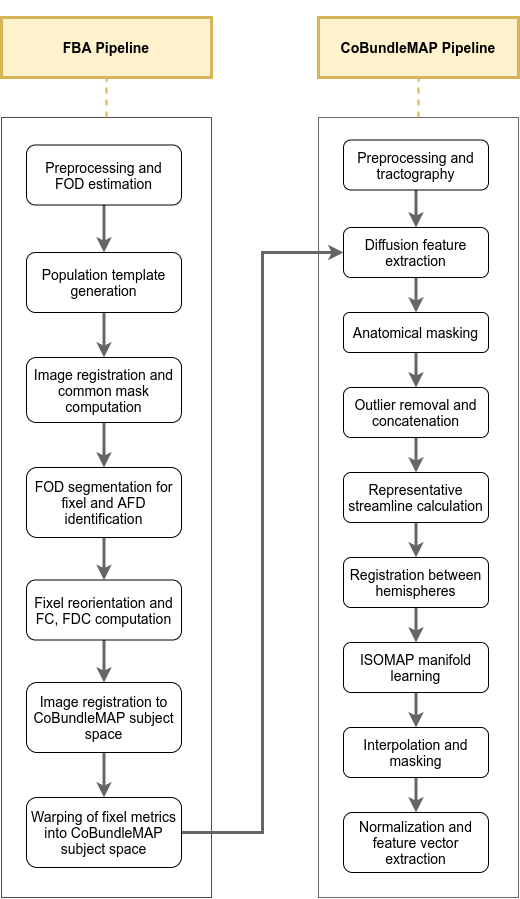
\includegraphics[width=11cm,keepaspectratio]{thesis_radomskyi/images/resulting-pipeline-diagram.png}
  \caption{\textbf{Schematic representation of the combined pipeline}}
  \label{fig:resulting-pipeline-diagram}
\end{figure}

%\label{ch:method} 

\end{document}

